\pdfoutput=1
\documentclass[conference]{IEEEtran}
%\documentclass[letter]{IEEEtran}
\usepackage{amsfonts}
\usepackage{graphicx}
\usepackage{color}
\usepackage{amsmath,amsfonts,amssymb,amsthm,epsfig,epstopdf,url,array}
\usepackage{url,textcomp}
%\usepackage{authblk}
\usepackage{cite}
\usepackage[misc]{ifsym}
\usepackage{verbatim}
\usepackage{subfigure}
\usepackage{caption}
\usepackage{algorithm}
\usepackage{algorithmicx}
\makeatletter
\newcommand\multiline[1]{\parbox[t]{\dimexpr\linewidth-\ALG@thistlm}{#1}}
\makeatother
\usepackage{algpseudocode}
\captionsetup[figure]{labelformat={default},labelsep=period,name={Fig.}}
%\usepackage[tbtags]{amsmath}
\newcommand{\bs}{\boldsymbol}
\newtheorem{theorem}{Theorem}
\newtheorem{lemma}{Lemma}
\newtheorem{corollary}{Corollary}
\newtheorem{mydef}{Definition}
\newtheorem{remark}{Remark}
\def\BibTeX{{\rm B\kern-.05em{\sc i\kern-.025em b}\kern-.08em
    T\kern-.1667em\lower.7ex\hbox{E}\kern-.125emX}}
\makeatletter
% \def \@IEEEauthorblocksetf {\IEEEauthorblockA\relax}
% \newcommand{\rmnum}[1]{\romannumeral #1}
% \newcommand{\Rmnum}[1]{\expandafter\@slowromancap\romannumeral #1@}
\makeatother

\begin{document}
\IEEEoverridecommandlockouts
\title{Graph Convolutional Network Enabled Power-Constrained HARQ Strategy for URLLC}

\author{
\IEEEauthorblockN{Yi~Chen\IEEEauthorrefmark{1},
        Zheng~Shi\textsuperscript{\Letter}\IEEEauthorrefmark{1},
        %Qingping Dou Xiaofang~Li
        Hong~Wang\IEEEauthorrefmark{2},
        Yaru~Fu\IEEEauthorrefmark{3},
        Guanghua~Yang\IEEEauthorrefmark{1},
        Shaodan Ma\IEEEauthorrefmark{4},
       and Haichuan Ding\IEEEauthorrefmark{5}}\\
\IEEEauthorrefmark{1}School of Intelligent Systems Science and Engineering, Jinan University, Zhuhai 519070, China.\\
\IEEEauthorrefmark{2}School of Communication and Information Engineering, Nanjing University of Posts and Telecommunications, \\Nanjing 210003, China.\\
\IEEEauthorrefmark{3}School of Science and Technology, Hong Kong Metropolitan University, Hong Kong SAR, China .\\
\IEEEauthorrefmark{4}The State Key Laboratory of Internet of Things for Smart City, University of Macau, Macau.\\
\IEEEauthorrefmark{5}School of Cyberspace Science and Technology, Beijing Institute of Technology, Beijing 100081, China.
\thanks {This work was supported in part by National Natural Science Foundation of China under Grants 62171200, 62171201, and 62261160650, in part by Guangdong Basic and Applied Basic Research Foundation under Grant 2023A1515010900, in part by Zhuhai Basic and Applied Basic Research Foundation under Grant ZH22017003210050PWC, in part by the Hong Kong Research Matching Grant (RMG) in the Central Pot under Project No. CP/2022/2.1, in part by the Major Talent Program of Guangdong Provincial under Grant 2019QN01S103, in part by the Science and Technology Development Fund, Macau SAR under Grants 0087/2022/AFJ and SKL-IOTSC(UM)-2021-2023, and in part by Open Research Foundation of National Mobile Communications Research Laboratory of Southeast University under Grant 2023D01. (\emph{Corresponding Author: Zheng Shi.})}
}

\maketitle
% Note that keywords are not normally used for peerreview papers.
\begin{abstract}
%We consider the problem of power allocation using HARQ-IR over time-correlated fading channels, where the transmitter has only statistical channel state information. Through the optimization of the transmission power, the throughput is maximized under the constraints of the power sum and the outage probability at the same time when the transmission rate is fixed. We model the multiple transmission process of HARQ as a graph structure through the graph neural network theory, embed the channel correlation as the edge features between nodes in the graph, and use the graph neural network to learn the topological structure information of the graph to determine the power allocation result . Simulation results verify that HARQ-IR can achieve higher throughput than other HARQ schemes
In this paper, a power-constrained hybrid automatic repeat request (HARQ) transmission strategy is developed to support ultra-reliable low-latency communications (URLLC). In particular, we aim to minimize the delivery latency of HARQ schemes over time-correlated fading channels, meanwhile ensuring the high reliability and limited power consumption. To ease the optimization, the simple asymptotic outage expressions of HARQ schemes are adopted. Furthermore, by noticing the non-convexity of the latency minimization problem and the intricate connection between different HARQ rounds, the graph convolutional network (GCN) is invoked for the optimal power solution owing to its powerful ability of handling the graph data. The primal-dual learning method is then leveraged to train the GCN weights. Consequently, the numerical results are presented for verification together with the comparisons among three HARQ schemes in terms of the latency and the reliability, where the three HARQ schemes include Type-I HARQ, HARQ with chase combining (HARQ-CC), and HARQ with incremental redundancy (HARQ-IR). To recapitulate, it is revealed that HARQ-IR offers the lowest latency while guaranteeing the demanded reliability target under a stringent power constraint, albeit at the price of high coding complexity.

\end{abstract}
\begin{IEEEkeywords}
Graph neural networks, HARQ-IR, power allocation, time-correlated fading channels
\end{IEEEkeywords}

\IEEEpeerreviewmaketitle
\section{Introduction}\label{sec:intro}
%\textcolor[rgb]{1.00,0.00,0.00}{show the challenges}
\IEEEPARstart Nowadays, ultra-reliable low-latency communications (URLLC) have become an unprecedented paradigm shift to support the mission-critical internet-of-things (IoT) applications \cite{9826826}. For instance, as per the 3rd generation partnership project (3GPP), a 32 byte packet is expected to transmit within 1 ms along with a reliability of at least 99.999\%. To confront this stringent requirement, hybrid automatic repeat request (HARQ) is one of the key enabling technologies that provide reliable transmissions to combat channel fading. On the basis of different encoding and decoding techniques, HARQ can be divided into three types, namely Type-I HARQ, HARQ with chase combining (HARQ-CC), and HARQ with incremental redundancy (HARQ-IR). In essence, HARQ sacrifices the delay performance to improve reliability, which inevitably hinders its widespread applications in supporting URLLC. To overcome this shortcoming, HARQ should be properly designed with more flexibility to accommodate diverse requirements of latency and reliability.

%In the HARQ scheme, the transmitter judges whether to send the next new message or retransmit the old message according to the decoding feedback of the receiver.


%the effective use of HARQ scheme helps to achieve the low error rate requirements of URLLC, however the use of time diversity to combat channel impairment will naturally increase the delay,

%in order to meet the extreme needs of URLLC for the two opposing requirements, in the resource allocation for complex wireless network environment to provide efficient and intelligent resource allocation algorithm has become imminent.

%In order to meet the high reliability and low-latency requirements

%Compared to the fourth generation (4G) systems such as Long Term Evolution (LTE), which focuses on mobile bandwidth, the fifth generation (5G) systems add support for massive machine-type communications (mMTC) and ultra-reliable low-latency communications(URLLC) to face the urgent needs of massive interactive devices and high-performance computing applications.
%As an unprecedented feature,

%URLLC support for mission-critical services is an important highlight of 5G, and 3GPP gives general requirements for reliability and latency, i.e., the delay of each transmission of $32$ bytes and the block error rate (BLER) are less than $1$ms and 10e-5, respectively.
%The challenge for URLLC is to juggle these two opposing and demanding needs at the same time.


%With only statistical channel state information at the transmitter, many

%especially for  and rate selection \cite{7247293}, leading many scholars to conduct in-depth research on it.
%When the transmitter only learns limited or statistical CSI, reasonable and effective allocation of resources for HARQ can further optimize the transmission capacity of the system,


 %The traditional radio resource allocation schemes in HARQ can be divided into two categories, the first one is to seek the closed solution of the optimization problem,
 %In \cite{7247293}, the author first deduces the delay-limited throughput (DLT) of the cooperative HARQ-CC scheme under the time-correlated channel, and selects the optimal rate by maximizing the DLT through the golden section search.
The optimal design of HARQ schemes has been extensively studied in the literature. To name a few, in \cite{6697940}, the outage probability of HARQ-CC was minimized by imposing a constraint on the average power consumption. The asymptotic outage probability was used to enable the optimal power allocation with geometric programming (GP). The similar method was then applied to solve the minimization of the expected energy consumption for HARQ-IR given a maximum allowable outage tolerance in \cite{9473556}. Moreover, in \cite{8362650}, the goodput of HARQ-IR was maximized through the joint optimization of the transmission powers and transmission rate under an average power constraint. The joint optimization of powers and rate was further considered to maximize the energy efficiency of HARQ schemes, which were solved in closed-form with the Karush-Kuhn-Tucker (KKT) conditions. Furthermore, the optimization of various HARQ-assisted systems has also received considerable research interest lately. To be specific, the power efficient design was considered for HARQ-CC aided non-orthgonal multiple access (NOMA) systems in \cite{9089002}, wherein successive convex approximation (SCA) was used to provide the optimal power solution. HARQ-NOMA-assisted short packet communications were investigated in \cite{9211722}, where a genetic algorithm was applied to optimize the power levels in power-constrained and reliability-constrained scenarios. %the user's packet error rate (PER) as well as throughput are analyzed by Markov models, followed by
%genetic algorithm was utilized to minimize the packet error rate and solve the minimum required block length problem for power-constrained and reliability-constrained scenarios, respectively.
Apart from high reliability and limited power consumption, the guarantee of low latency is also of profound significance to realize URLLC, while this topic was rarely examined except in a few existing works. Particularly,
%{\color{red}Please cite some references in these three years rather than long long ago!!! around three references related to HARQ-assited systems, better journal papers!}....
in \cite{10015032}, the age of information (AoI) was minimized for HARQ-IR-assisted multi-RIS systems while ensuring power and outage constraints. %, which alternatively optimizes the transmit rate and power to minimize under the premise of optimal phase dependent priority determination.
In addition, the authors in \cite{9606298} maximized the overall rates of enhanced mobile broadband (eMBB) users in HARQ-assisted grant free systems under the constraint of a maximum tolerable probability of delay bound violation. However, independent fading channels were generally assumed in these works \cite{9473556, 9089002, 9211722, 10015032, 9606298} whose results are inapplicable to the correlated fading channels. Due to the frequent occurrence of time-selective fading channels, there is an urgent need to propose a proper latency assurance strategy for HARQ schemes over correlated fading channels. % were seldom incorporated into the optimal design of HARQ systems in the existing works.
%However, the performance analysis metrics such as outage probability/block error rate are based on simulation or approximate results, and lack precise close-form expressions, and even if expressions can be derived in special cases, their structural forms are generally too complex to provide accurate guidance for subsequent system optimization design. In addition, optimization problems involving resource allocation, such as maximizing throughput and minimizing outage probability, are usually complex and non-convex, making the optimization of design work significantly more difficult, difficult or even impossible to optimize the results.
 %In \cite{9089002}, for the non-convex outage probability problem, the authors use a successive convex approximation (SCA) based algorithm for continuous approximation, and iteratively updates the optimization scheme.
 %\cite{8319455} deduces the brief outage probability expressions of the three HARQ schemes respectively, and jointly optimizes the power allocation and rate selection by solving the closed solution under the condition of satisfying the Qos constraint. In order to maximize the DLT in MISO time-correlated Rayleigh fading channels, the author in
  %Similarly, in order to perform optimal power allocation, in \cite{6697940} the author transforms the non-convex problem into a convex geometric programming problem (GPP) problem by approximating the outage probability, and uses the primal-dual interior point method to solve it effectively.
 %HARQ-IR geometric programming (GP) is utilized to solve power  \cite{9473556} minimize the expected energy consumption of wireless transmission given the outage probability constraint and the maximum average number of retransmissions.
% In \cite{8362650}, the author decomposes the performance index Goodput maximization problem of the HARQ scheme into a univariate optimization problem through decomposition theory, and optimizes the transmit power and transmission rate by solving the closed solution of the optimization problem. Considering the energy efficiency maximization problem, the author in
 %\cite{6364609} uses the lognormal distribution to approximate the DLT equation in HARQ-CC, and find the closed solution of the optimal rate and power allocation.
 %In \cite{5669231} the author considers the resource usage of signaling overhead, and proposes a rate selection scheme for continuous scheduling in time-correlated Nakagami-m fading channels under given Qos requirements.
% The other is to transform it into a convex problem.

% According to shown in \cite{8319455,book01}, the combined HARQ-IR scheme can achieve higher throughput due to the introduction of additional coding gain than the HARQ-CC as well as type-I schemes, then the study in this paper focuses on the HARQ-IR scheme.

%this will inevitably lead to an extremely short time interval between two transmissions, and its time correlation becomes an important factor affecting transmission performance. It is naturally embedded as a graph neural network network theory  \cite{xu20181111} connectivity representation between graph structure nodes, At the same time, a classic idea to improve system performance is to integrate prior knowledge \cite{9743856}, that is, to combine the structural design of the neural network with the target task system structure to be processed in the scene \cite{9252917}. In this paper, we propose to transform the correlation between multiple transmission events in HARQ-IR transmission and the channels during transmission into nodes and edges in a graph structure, and use graph neural networks as an intermediate structure for parameter optimization to jointly optimize the transmit power for each transmission event.
%In order to minimize the delivery latency while guaranteeing the high reliability, this paper proposes a power-constrained HARQ strategy with the statistical channel state information (CSI) available at the transmitter. The simple asymptotic outage expressions of HARQ schemes are adopted to avoid heavy computational burden. However, the optimization problem still cannot be easily solved with the off-the-shelf tools due to its complex formulation, which inspires us to resort to artificial intelligence (AI) techniques. By taking into account that the transmit power allocated in the current HARQ round is commonly independent of the subsequent HARQ rounds, it is natural to come up with graph neural networks to capture this special structure. The graph convolutional network (GCN) is then invoked for the optimal power allocation by treating different HARQ rounds and channel correlation as graph nodes and edges, respectively. The trainable GCN weights are updated by using primal-dual learning approach. Finally, the GCN-based stra three HARQ schemes in terms of the latency and the reliability are compared , where the three HARQ schemes include Type-I HARQ, HARQ with chase combining (HARQ-CC), and HARQ with incremental redundancy (HARQ-IR). Last but not least, it is revealed that HARQ-IR offers the lowest latency while guaranteeing the demanded reliability target under a stringent power constraint, albeit at the price of high coding complexity.

In order to minimize the delivery latency while guaranteeing the high reliability, this paper proposes a power-constrained HARQ strategy by considering time-correlated fading channels. The simple asymptotic outage expressions of HARQ schemes are adopted to avoid heavy computational burden. Unfortunately, the optimization problem still cannot be easily solved by  using the off-the-shelf tools due to the fractional objective function and non-convex constraints. This has inspired us to explore the use of artificial intelligence (AI) techniques. By taking into account that the transmit power allocated in the current HARQ round is affected by the previous HARQ rounds regardless of the subsequent HARQ rounds, and the time correlation takes place among fading channels, it is natural to come up with graph neural networks to capture this special transmission structure. The graph convolutional network (GCN) is then invoked for the optimal power allocation of HARQ by treating different HARQ rounds and channel correlation as graph nodes and edges, respectively. The trainable GCN weights are updated by using primal-dual learning approach. Finally, the latency and the reliability performance of the GCN-enabled power allocation strategy for three HARQ schemes was investigated through numerical experiments, where the three HARQ schemes include Type-I HARQ, HARQ-CC, and HARQ-IR. Last but not least, despite its high coding complexity, HARQ-IR can provide the lowest latency while ensuring reliable performance within strict power constraints.


%the cannot be affected by the subsequent transmissions, this special structure can be captured by GCN...
%In this paper, the graph convolutional network (GCN) enabled power-constrained hybrid automatic repeat request (HARQ) schemes are developed to support ultra-reliable low-latency communications (URLLC). In particular, we aim to minimize the delivery latency of HARQ schemes To ease the optimization, the simple asymptotic outage expressions of HARQ schemes are adopted.
%Furthermore, by noticing the non-convexity of the latency minimization problem and the intricate connection between different HARQ rounds,

The rest of the paper is structured as follows. Section \ref{sec:model} elaborates on the system model and formulates the latency minimization problem for power-constrained HARQ schemes. In Section \ref{sec:gcnmodel}, a GCN-enabled power allocation strategy is designed to solve the optimization problem. Section \ref{sec:EXPERIMENTS} verifies the effectiveness of the proposed strategy through numerical experiments. Finally, concluding remarks are drawn in Section \ref{sec:CONC}.
\section{System Model}\label{sec:model}
This paper considers a point-to-point HARQ-aided URLLC system. To begin, the system model is delineated in this section, including HARQ schemes, signal transmission model, and problem formulation.
\subsection{HARQ Schemes}
HARQ can be classified into three categories according to different coding operations, including Type-I HARQ, HARQ-CC, and HARQ-IR. More specifically, for both Type-I HARQ and HARQ-CC, the same codeword is delivered in all HARQ rounds. At the receiver side, Type-I HARQ decodes its message by solely relying on the currently received codeword, while HARQ-CC combines the erroneously received codewords for maximal-ratio combining (MRC). Undoubtedly, HARQ-CC outperforms Type-I HARQ due to the fact that even the failed packets contain useful information. Unlike Type-I HARQ and HARQ-CC, HARQ-IR transmits codewords with different redundancy among all HARQ rounds. Hence, a long codeword is first chopped into several sub-codewords at the transmitter, which will be sent one by one upon retransmission request. At the receiver, the previously received codewords are then concatenated to form a long codeword for the joint decoding. Owing to the high encoding/decoding complexity, HARQ-IR achieves the superior performance of reliability.

%In HARQ-IR a piece of information is divided into $K$ sub-codewords of equal length, where $K$ represents the maximum number of transmissions allowed to send this message. After each transmission, the currently received codeword is combined with the previously received erroneous codeword for decoding. If the decoding is successful, an acknowledgement (ACK) will be sent to the sender and the transmission of the next message will begin. If the decoding fails, a negative acknowledgement(NACK) will be returned, and the next sub-codeword will be sent until the number of transmissions $K$ is reached. Fig. \ref{FIG1} shows a HARQ-IR transmission process with a maximum number of transmissions of 4.


\begin{figure}[htbp]
    \centering
    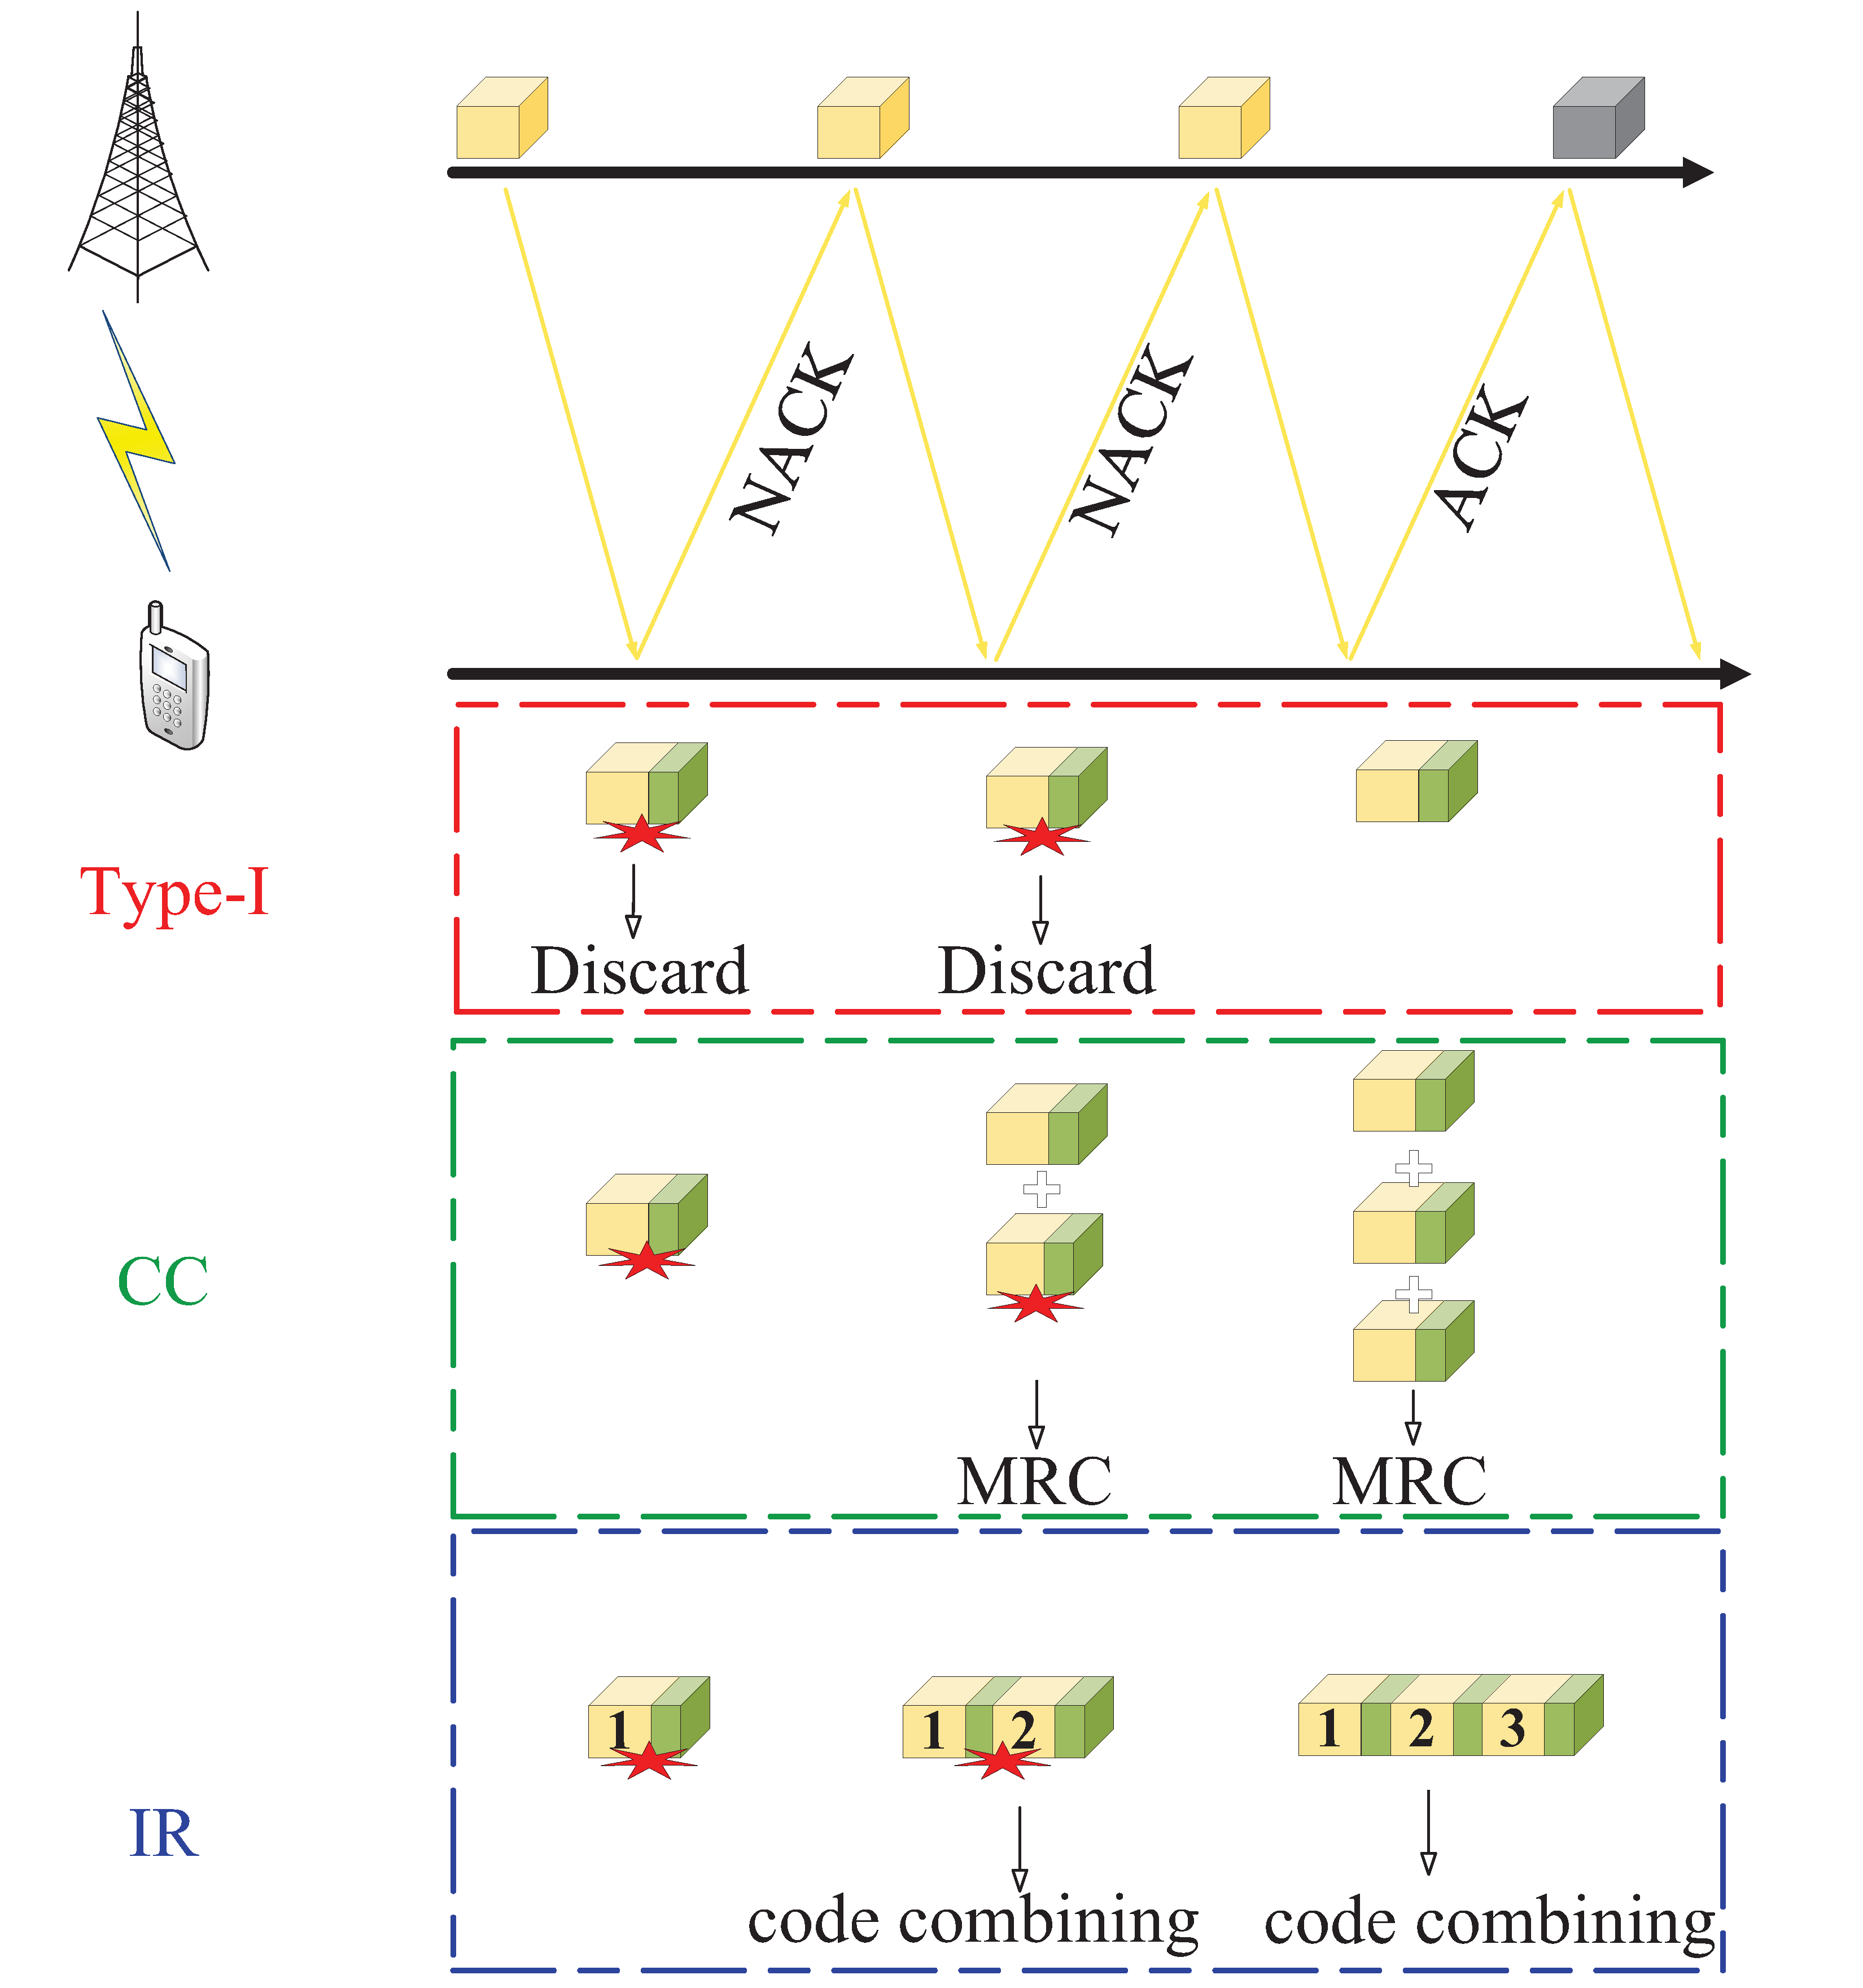
\includegraphics[width=8cm]{HARQSchme4.eps}
    \caption{An example of HARQ transmissions.}
    \label{FIG1} %ÓÃÓÚÎÄÄÚÒýÓõıêÇ©
\end{figure}

\subsection{Signal Transmission Model}
By considering blocking fading channels, the received signal in the  $k$-th HARQ round can be expressed as
\begin{equation}\label{eqn:receive signal}
{{\bf{y}}_k} = {h_k}{{\bf{x}}_k} + {{\bf{n}}_k},
\end{equation}
where ${{\bf{x}}_k}$ denotes the $k$-th codeword of length $M$ with average power $p_k$, and ${{\bf{n}}_k}$ denotes a complex additive white Gaussian noise vector with zero mean vector and identity covariance matrix, i.e., ${{\bf{n}}_k} \sim {\cal CN}({\bf 0},{{\bf{I}}_{ M}})$ %${{\bf{I}}_L}$ represents an identity matrix,
,
${h_k}$ refers to the channel coefficient of the $k$-th transmission. To avoid large transmission latency under unfavorable fading channels, the maximum number of HARQ rounds for sending each message is limited up to $K$. Due to the frequent occurrence of the correlation among fading channels \cite{5692978}, the time-correlated Rayleigh fading channels are used to model $h_k$ as
\begin{equation}\label{eqn:channel model}
{h_k} = {\xi    _k}\left(\sqrt {1 - {\rho ^{2(k + \delta  - 1)}}} {\alpha _k} + {\rho ^{k + \delta  - 1}}{\alpha _0}\right),
\end{equation}
where the factor $\rho$ measures the intensity of the time correlation between channel coefficients, $\delta$ and $ {\xi _k}^2$ denote the feedback delay and the average power of the channel, respectively, ${\alpha _0},{\alpha _1},...,{\alpha _k}$ are mutually independent and obey complex normal distributions with zero mean and unit variance.%, i.e., ${\alpha _0},{\alpha _1},\cdots, {\alpha _K} \sim {\cal CN}(0,1)$

According to \eqref{eqn:receive signal}, the received signal-to-noise ratio (SNR) in the $k$-th transmission can be obtained as
\begin{equation}\label{eqn:SNR}
{\gamma _k} = {p_k}{\left| {{h_k}} \right|^2}, \, k\in [1,K], %= {P_k}{\sigma _k}^2{\left| {\sqrt {1 - {\rho ^{2(k + \delta  - 1)}}} {\alpha _k} + {\rho ^{k + \delta  - 1}}{\alpha _0}} \right|^2}
\end{equation}
where ${p_k}$ denotes the average transmit power in the $k$-th HARQ round. %Since the channel magnitude $\left| {{h_k}} \right|$ is Rayleigh distributed, ${\gamma _k}$ compiles with exponential distribution with mean ${p_k}{\sigma _k}^2$, Due to the correlation between fading channels, the SNRs $\gamma  = ({\gamma _1},{\gamma _2},...,{\gamma _K})$ are thus correlated exponential RVs.

%\subsection{Performence Metric}




\subsection{Problem Formulation of Power-Constrained HARQ for URLLC}
%In some URLLC scenarios, when IoT devices are usually at the edge of the network, decisions need to be made according to the special scenario. For example, in applications such as smart medical testing \cite{9439861} and industrial IoT \cite{8792078}, ,9089244,8673568
The mission-critical IoT applications usually emphasize stringent constraints of reliability and latency \cite{9810267}. Besides, the IoT devices  are frequently equipped with non-rechargeable battery which cannot provide continuous power supply. The energy consumption of IoT networks mainly comes from the radio frequency communication module. Hence, the transmit powers should be optimally devised to prolong the lifetime of IoT networks. In this paper, we aim at the accommodation of low latency as well as high reliability via the power allocation in different HARQ rounds. To proceed, we denote by $N_b$ and $B$ the total number of information bits and the bandwidth, respectively. The delivery latency of these information bits is thus calculated as
\begin{equation}\label{eqn:delay_def}
\tau = \frac{N_b}{\eta B},
\end{equation}
where $\eta$ denotes the effective spectral efficiency. The spectral efficiency of HARQ scheme can be estimated by using the long term average throughput (LTAT) of HARQ, which can be obtained as \cite{6879267}
\begin{equation}\label{eqn:throught2}
\eta  = \frac{{R(1 - {P_{out,K}})}}{{1 + \sum\limits_{k=1}^{K - 1} {{P_{out,k}}} }},
\end{equation}
where $R = b/M$ and $b$ denote the preset transmission rate  and the number of original information bits, respectively. In addition, $P_{out,k}$ refers to the outage probability after $k$ HARQ rounds. With the definition of the latency, the latency minimization problem of the power-constrained HARQ while guaranteeing its high reliability can be formulated as
% the end device may have a finite amount of energy available for each message during communication, this requires that the average power allocated to transmit using the HARQ scheme is less than a given threshold to minimize the transmission delay while ensuring reliability, which can be expressed as.
\begin{equation}\label{eqn:min_delay}
\begin{array}{*{20}{cl}}
{\mathop {\min }\limits_{{p_1}, \cdots ,{p_K}} }&\tau \\
{\rm s.t.}&{{P_{out,K}} \le \varepsilon },\\
{}&{p_{\rm avg} \le \bar p,}
\end{array}
\end{equation}
where the reliability is ensured by imposing a constraint on the outage probability, and $\varepsilon$ denotes the maximum acceptable outage tolerance, ${\bar p}$ denotes the maximum allowable total transmit power, and $p_{\rm avg}$ denotes the average transmit power that is evaluated as
\begin{equation}
    p_{\rm avg} = \sum\limits_{k = 1}^K {{p_k}{P_{out,k - 1}}},
\end{equation}
and we stipulate $P_{out,0} = 1$. It should be mentioned that the power allocation is optimally designed by only utilizing the statistical channel state information (CSI) to avoid frequent signaling interactions and conserve time.


%Accordingly, the latency maximization of the power-constrained HARQ
%where . Through the observation of formula (\ref{eqn:delayexep}), we found that when the fixed size information is transmitted, the delay $\tau$ is a negative correlation function related to the  LTAT $\eta$, and the maximization of the throughput in the formula (\ref{eqn:throught2}) is equivalent to the minimization of the delay process, so (\ref{eqn:min delay}) can be reformulated as:
%\begin{equation}\label{eqn:max throughtput}
%\begin{array}{*{20}{c}}
%{\max }&\eta \\
%%{}&{\sum\limits_{k = 1}^K {{p_k}{p_{out,k - 1}} \le \bar P.} }
%\end{array}
%\end{equation}
%\subsubsection{Outage Probability}
%Specifically, assuming that information-theoretic capacity achieving channel coding is adopted for HARQ-IR, an outage event happens when the accumulated mutual information ${I_k}$ is below the transmission rate $R$. The outage probability after $K$ transmissions is thus written as
%\begin{equation}\label{eqn:outage probability1}
%{p_{out,K}} = \Pr ({I_k} < R)
%\end{equation}
%\subsubsection{Long Term Average Throughput}
%If we need to transmit $B$ bits of information, according to (\ref{eqn:throught2}) of throughput, we can get an expression about delay $\tau $ as
%\begin{equation}\label{eqn:delayexep}
%\tau  = \frac{B}{\eta }
%\end{equation}
%\subsubsection{Average Transmission Power}
%When the power at one end of the transmitter is limited, the power to be allocated may satisfy certain constraints:
%\begin{equation}\label{eqn:powerlimited}
%\begin{array}{l}
%\sum\limits_{k = 1}^K {{p_k}{p_{out,k - 1}} \le \bar P }
%\end{array}
%\end{equation}
%where
\section{GCN-Enabled Power Allocation Strategy}\label{sec:gcnmodel}
% Prior to the power allocation, this section describes the graph neural network model, including the representation of the graph network and the basic theory of the graph neural network
Although the exact outage expressions of HARQ systems were derived in \cite{7448651,7833558,7959548}, the outage expressions involve the summation of an infinite number of special functions. Such complex representations entail a high computational burden for the optimal design. In order to overcome this issue, the asymptotic expressions of the outage probabilities are leveraged in the optimal design. As derived in \cite{7448651,7833558,7959548}, the asymptotic outage probabilities of three types of HARQ schemes are given by %[{\color{red}{revise the equation below}}]
% \begin{equation}\label{eqn:pout_asy}
% \begin{array}{l}
% {P_{out,k}} \simeq {{\cal G}_K}({2^R}){({\cal L}(\rho ,K))^{ - 1}}\frac{1}{{\prod\limits_{k = 1}^K {{p_k}} \prod\limits_{k = 1}^K {{\sigma _k}^2} }},
% \end{array}
% \end{equation}
% where $\rho \ne 1$....
\begin{equation}\label{eqn:pout_asy}
{P_{out,K}} = \left\{ {\begin{array}{*{20}{c}}
{{\varsigma _K}{{({2^R} - 1)}^K},}&{{\rm{Type-I}}}\\
{{\varsigma _K}{{({2^R} - 1)}^K}/K!,}&{{\rm{CC}}}\\
{{\varsigma _K}{\mathcal G_K}(R),}&{{\rm{IR}}}
\end{array}} \right.,
\end{equation}
where $\Gamma \left(  \cdot  \right)$ denotes the Gamma function, % ${\varsigma _K}$ defines the effect of time-correlated fading channels,
${\varsigma _K} = \frac{{{{\left( {\ell\left( {\rho ,K} \right)} \right)}^{ - 1}}}}{{\prod\nolimits_{k = 1}^K {{p_k}{\xi _k}^2} }}$, ${\ell}(\rho ,K)$ quantifies the effect of correlation that is given by
\begin{equation}\label{eqn:L_func}
\begin{array}{l}
{\ell}(\rho ,K) = \left(1 + \sum\limits_{k = 1}^K {\frac{{{\rho ^{2(k + \delta  - 1)}}}}{{1 - {\rho ^{2(k + \delta  - 1)}}}}} \right)\prod\limits_{k = 1}^K {\left(1 - {\rho ^{2(k + \delta  - 1)}}\right)},
\end{array}
\end{equation}
it should be noted that $\rho \ne 1$, and $\mathcal G_K(R)$ reads as
\begin{equation}\label{eqn:g_func}
\begin{array}{l}
{{\cal G}_K}(R) = {( - 1)^K} + {2^R}\sum\limits_{k = 0}^{K - 1} {{{( - 1)}^k}\frac{{{{(R\ln 2)}^{K - k - 1}}}}{{(K - k - 1)!}}}.
\end{array}
\end{equation}

Unfortunately, due to the correlation among different transmissions, the fractional form of the objective function, and non-convexity of constraints, the optimization problem in \eqref{eqn:min_delay} still cannot be easily solved by means of the classical optimization methodologies, such as CVX tools. The success of the application of GCNs in power allocation policy learning for wireless networks \cite{9252917} has motivated us to develop GCN-based power allocation for power-constrained HARQ schemes. It is clear that different HARQ rounds and correlations among them can be represented by graph nodes and edges, respectively. %({\color{red}The observation that different HARQ rounds and their correlation can be modeled as graph nodes and edges, coupled with the successful deployment of GCN in power allocation policy learing for wireless networks\cite{9252917}, propels us to advance GCN-based approaches to power allocation for power-limited HARQ schemes.})
It is noteworthy that GCN is suitable herein due to its ability of exploiting the graph structure to process data. In what follows, a GCN-enabled power allocation scheme is detailed.
%Even if the asymptotic results can significantly reduce the computational complexity,
%To maximize the object function of (\ref{eqn:max throughtput}), we need to select the optimal power allocation result.
%However, the objective function is a complex fractional form and non-convex, and it is more difficult to go deeper with the exact outage probability optimization problem. Even if the asymptotic outage probability is used, the traditional method of seeking a closed solution or by converting it into a convex problem iterative optimization methods require a huge amount of calculation, which constantly prompts us to seek a more efficient and reasonable method to face such problems. In order to make this maximization problem easy to handle, by deeply exploring the internal relationship between HARQ-IR transmission events , we found that it can be perfectly mapped to the graph structure for modeling representation.
%\eqref{eqn:min delay}
\subsection{GCN-Based Power Allocation}
%In order to facilitate the subsequent optimization design, the outage probability ${p_{out,K}}$ adopts the asymptotic result in the paper

%edges represented by correlations among fading channels
To enable the GCN-based power allocation, each HARQ round is modeled as a graph node. Moreover, as aforementioned that the statistical CSI is used, the graph edges can be characterized by the correlation coefficients among fading channels. More specifically, the channel correlation coefficient matrix ${\bf H}$ is calculated as
\begin{equation}\label{eqn:H_def_co}
    {\bf H} = %\left[  \left(\frac{{{\rm{E}}\left\{ {{h_i}^{\rm{H}}{h_j}} \right\}}}{{\sqrt {{\rm{E}}\left\{ {{{\left\| {{h_i}} \right\|}^2}} \right\}{\rm{E}}\left\{ {{{\left\| {{h_j}} \right\|}^2}} \right\}} }}\right)_{(i,j)} \right]_{1 \le i,j\le K},
    \left[  {\alpha}_{ij} \right]_{1 \le i,j\le K},
\end{equation}
where the element ${\alpha _{ij}} $ is
\begin{equation}
    {\alpha _{ij}} = \left\{ {\begin{array}{*{20}{c}}
{{\rm{E}}\left\{ {{h_i}^{*}{h_j}} \right\},}&{i \le j}\\
{0,}&{\rm else}
\end{array}} \right.,
\end{equation}
wherein the superscript ${*}$ denotes the complex conjugate operation and $\rm E\{\cdot\}$ is the expectation operation. The rationale of ${\alpha _{ij}}=0$ for $i>j$ is due to the fact the $j$-th HARQ round cannot be influenced by the $i$-th HARQ round. With the time-correlated channel model in \eqref{eqn:channel model}, the diagonal entries of ${\bf H}$ can be calculated as ${\rm{E}}\left\{ {{{\left\| {{h_i}} \right\|}^2}} \right\} = {\xi _i}^2$ and its off-diagonal entries are given by ${\rm{E}}\left\{ {{h_i}^{*}{h_j}} \right\} = {\xi _i}{\xi _j}{\rho ^{i + j + 2\delta  - 2}}$ \cite{6094281}. %Hence, from \eqref{eqn:H_def_co}, the diagonal entries of ${\bf H}$ are ${\xi _i}^2$, and its  are equal to ${\rho ^{i + j + 2\delta  - 2}}$.
Apparently, ${\bf H}$ can be treated as the adjacency matrix in the directed graph network.
%that More specifically, we model the $K$ transmissions in HARQ-IR into a complete graph with vertices and edges.Naturally, we embed the channel correlation between two transmissions as the connection relationship between two nodes in the graph structure,
%we can define the calculation of the direct and indirect relationship of the channel during transmission as  ${\alpha _i} = 1$ and ${\beta _{i,j}} = {\rm E}({h_i}^{\rm H}{h_j})$, thus we can define the adjacency matrix $H$ with the ${\alpha _i}$ as the diagonal entries and ${\beta _{i,j}}$ as off-diagonal entries, i.e.,${H_{i,i}} = {\alpha _i},{H_{i,j}} = {\beta _{i,j}}(i \ne j)$. we quoted  to facilitate the calculation of the result of ${\beta _{i,j}}$, then it can be expressed as

%\begin{align}\label{eqn:betaexep}
%{\beta _{i,j}} = {\rm E}\left\{{h_i}^{\rm H}{h_j}\right\}%\notag\\
%& = {\rho ^{i + j + 2\delta  - 2}}\sqrt {E({{\left| {{h_i}} \right|}^2})E({{\left| {{h_j}} \right|}^2})} \notag\\
%&
%= {\sigma _i\sigma _j\rho ^{i + j + 2\delta  - 2}}
%\end{align}

%According to our transmission characteristics, the whole system can be regarded as a directed graph, we can define a transmission event as a node in a graph, and define the matrix $H$ as the adjacency matrix in the graph network. As shown in the Fig. \ref{FIG2}, it shows the representation of modeling the $5$ HARQ-IR (re)transmission events in  as a graph structure.

For tractability, the power policy functional space ${\bf p} = ( {{p_1},{p_2},...,{p_K}} )$ is parameterized by using a graph neural networks. More specifically, the power allocation policy is defined as ${\bf p}({\bf H}) = \Psi({\bf H};{\bf W})$, where $\Psi$ represents a $L$-layer GCN with trainable weights ${\bf W}$. Instead of optimizing ${\bf p}$, the neural network parameters ${\bf W}$ need to be optimally determined through the primal-dual learning approach \cite{9072356}. As shown in Fig. \ref{FIG2}, a $L$-layer GCN structure for the power-constrained HARQ schemes with $K=5$ is given as an example. With the input ${\bf V}^{(0)} = \frac{\bar p}{K} {\bf 1}_K$ to $\Psi({\bf H};{\bf W})$, %Assuming that in $K$ transmissions, the power allocated is ${\bf p} = ( {{p_1},{p_2},...,{p_K}} )$, we propose to use graph Convolutional Network (GCN) to optimize (\ref{eqn:max throughtput}) and maximize the parameters of the neural network architecture.
the $(l+1)$-th layer features  ${\bf V}^{(l + 1)}$ of GCN are updated by following the layer-wise propagation rule as
\begin{equation}\label{eqn:GNNfunc}
{{\bf{V}}^{(l + 1)}} = \sigma_l\left({{\bf{D}}^{ - \frac{1}{2}}}{\bf{H}}{{\bf{D}}^{ - \frac{1}{2}}}{{\bf{V}}^{(l)}}{{\bf{W}}^{(l)}}\right),
\end{equation}
where ${\bf 1}_K$ stands for an all-ones column vector, ${{\bf{D}}} = {\rm diag}({\bf{H}})$ denotes the degree matrix, ${{\bf{V}}^{(l)}} \in {\mathbb R^{K\times n_{l}}}$ is the matrix of node features in the $l$-th layer, ${{\bf W}^{(l)}} \in \mathbb R^{n_l\times n_{l+1}}$ is the trainable weight matrix in the $l$-th layer, $\sigma _l( \cdot )$ defines the activation function. Accordingly, the output of the $L$-th layer of the GCN is our desired power allocation policy. %The number of layers $L$ used in our simulations, the dimensions $n$ of the hidden layers, and the activation functions $\sigma ( \cdot )$ used are further explained in Section \ref{sec:EXPERIMENTS}.
\subsection{Primal-Dual Learning Approach}
In order to train the neural network weights ${\bf W}$, the iterative primal-dual learning approach is applied in this paper. Moreover, by realizing that the maximum allowable outage probability is generally very low (e.g., $\varepsilon=10^{-2}$), we apply the logarithm transformation to the outage probability, i.e., $\log {P_{out,K}}$, in order to amplify the effect of the outage constraint and meanwhile accelerate learning and alleviate the over-fitting.
%It should be emphasized that in order to preserve the influence of the outage probability on the overall loss function, we use the $log$ function to ensure that the model is more reasonable.
By taking this transformation into consideration, the Lagrangian of problem \eqref{eqn:min_delay} is formulated as
%To treat the constraints in (\ref{eqn:max throughtput}), we formulate the Lagrangian dual problem by introducing nonnegative multipliers $\lambda  \ge 0$ and $\upsilon  \ge 0$. Then the Lagrangian is given by
\begin{multline}\label{eqn:dual prrobelm}
\mathcal L_{\Psi}({\bf{W}},\lambda ,\upsilon ) = \tau + \lambda (\log {P_{out,K}} - \log \varepsilon )\\
 + {\upsilon }\left(\sum\limits_{k = 1}^K {{p_k}{P_{out,k-1}}} - \bar p \right),
\end{multline}
where $\lambda  \ge 0$ and $\upsilon  \ge 0$ are the Lagrangian multiplier associated with the two constraints in problem \eqref{eqn:min_delay}. It is noteworthy that $\tau $, ${P_{out,K}}$, and $\bf p$ are the functions of the trainable parameters $\bf W$. According to the gradient descent algorithm, the neural network parameters $\bf W$ at step $s$ can be updated as

\begin{equation}\label{eqn:optweight}
\begin{array}{l}
{{\bf{W}}_{s + 1}} = {{\bf{W}}_s} - {\theta _{{\bf{W}},s}} {\nabla _{\bf{W}}}{{\rm E}_{\rho  \sim \mathcal A}}\left\{\mathcal L({{\bf{W}}_s},{\lambda_s} ,{\upsilon_s})\right\},
\end{array}
\end{equation}
where the term ${\theta _{{\bf{W}},s}}$ denotes the step size at the $s$-th iteration and the actual time correlation $\rho$ follows a certain distribution $\mathcal A$ within the range $[0,1)$. Besides, the multipliers are updated by capitalizing on the sub-gradient method as
%Following standard primal-dual solutions of optimization problems \cite{1664999, 9747764}, this Lagrangian motivates the following iterative primal dual learning approach:
\begin{equation}\label{eqn:optstepa}
%{{\bf{W}}_{s + 1}} = {{\bf{W}}_s} + {\theta _{{\bf{W}},s}}{\nabla _{\bf{W}}}L({\bf{W}},\lambda ,\upsilon )\\
{\lambda _{s + 1}} = {\left[ {{\lambda _s} + {\theta _{{\lambda },s}}({{\rm E}_{\rho  \sim \mathcal A}}\left\{\log ({P_{out,K}})\right\} - \log (\varepsilon))} \right]_ + },
\end{equation}

\begin{equation}\label{eqn:optstepb}
{\upsilon _{s + 1}} = {\left[ {{\upsilon _s} + {\theta _{{\upsilon },s}}({{\rm E}_{\rho  \sim \mathcal A}}\left\{p_{\rm avg}\right\} - \bar p)} \right]_ + },
\end{equation}
where ${\theta _{{\lambda },s}}$ and ${\theta _{{\upsilon },s}}$ correspond to the step sizes, and $[x]_+ = \max\{0,x\}$. The pseudocode of GCN-based power allocation scheme is shown in Algorithm \ref{alg:algor1}.


\begin{figure}[htbp]
    \centering
    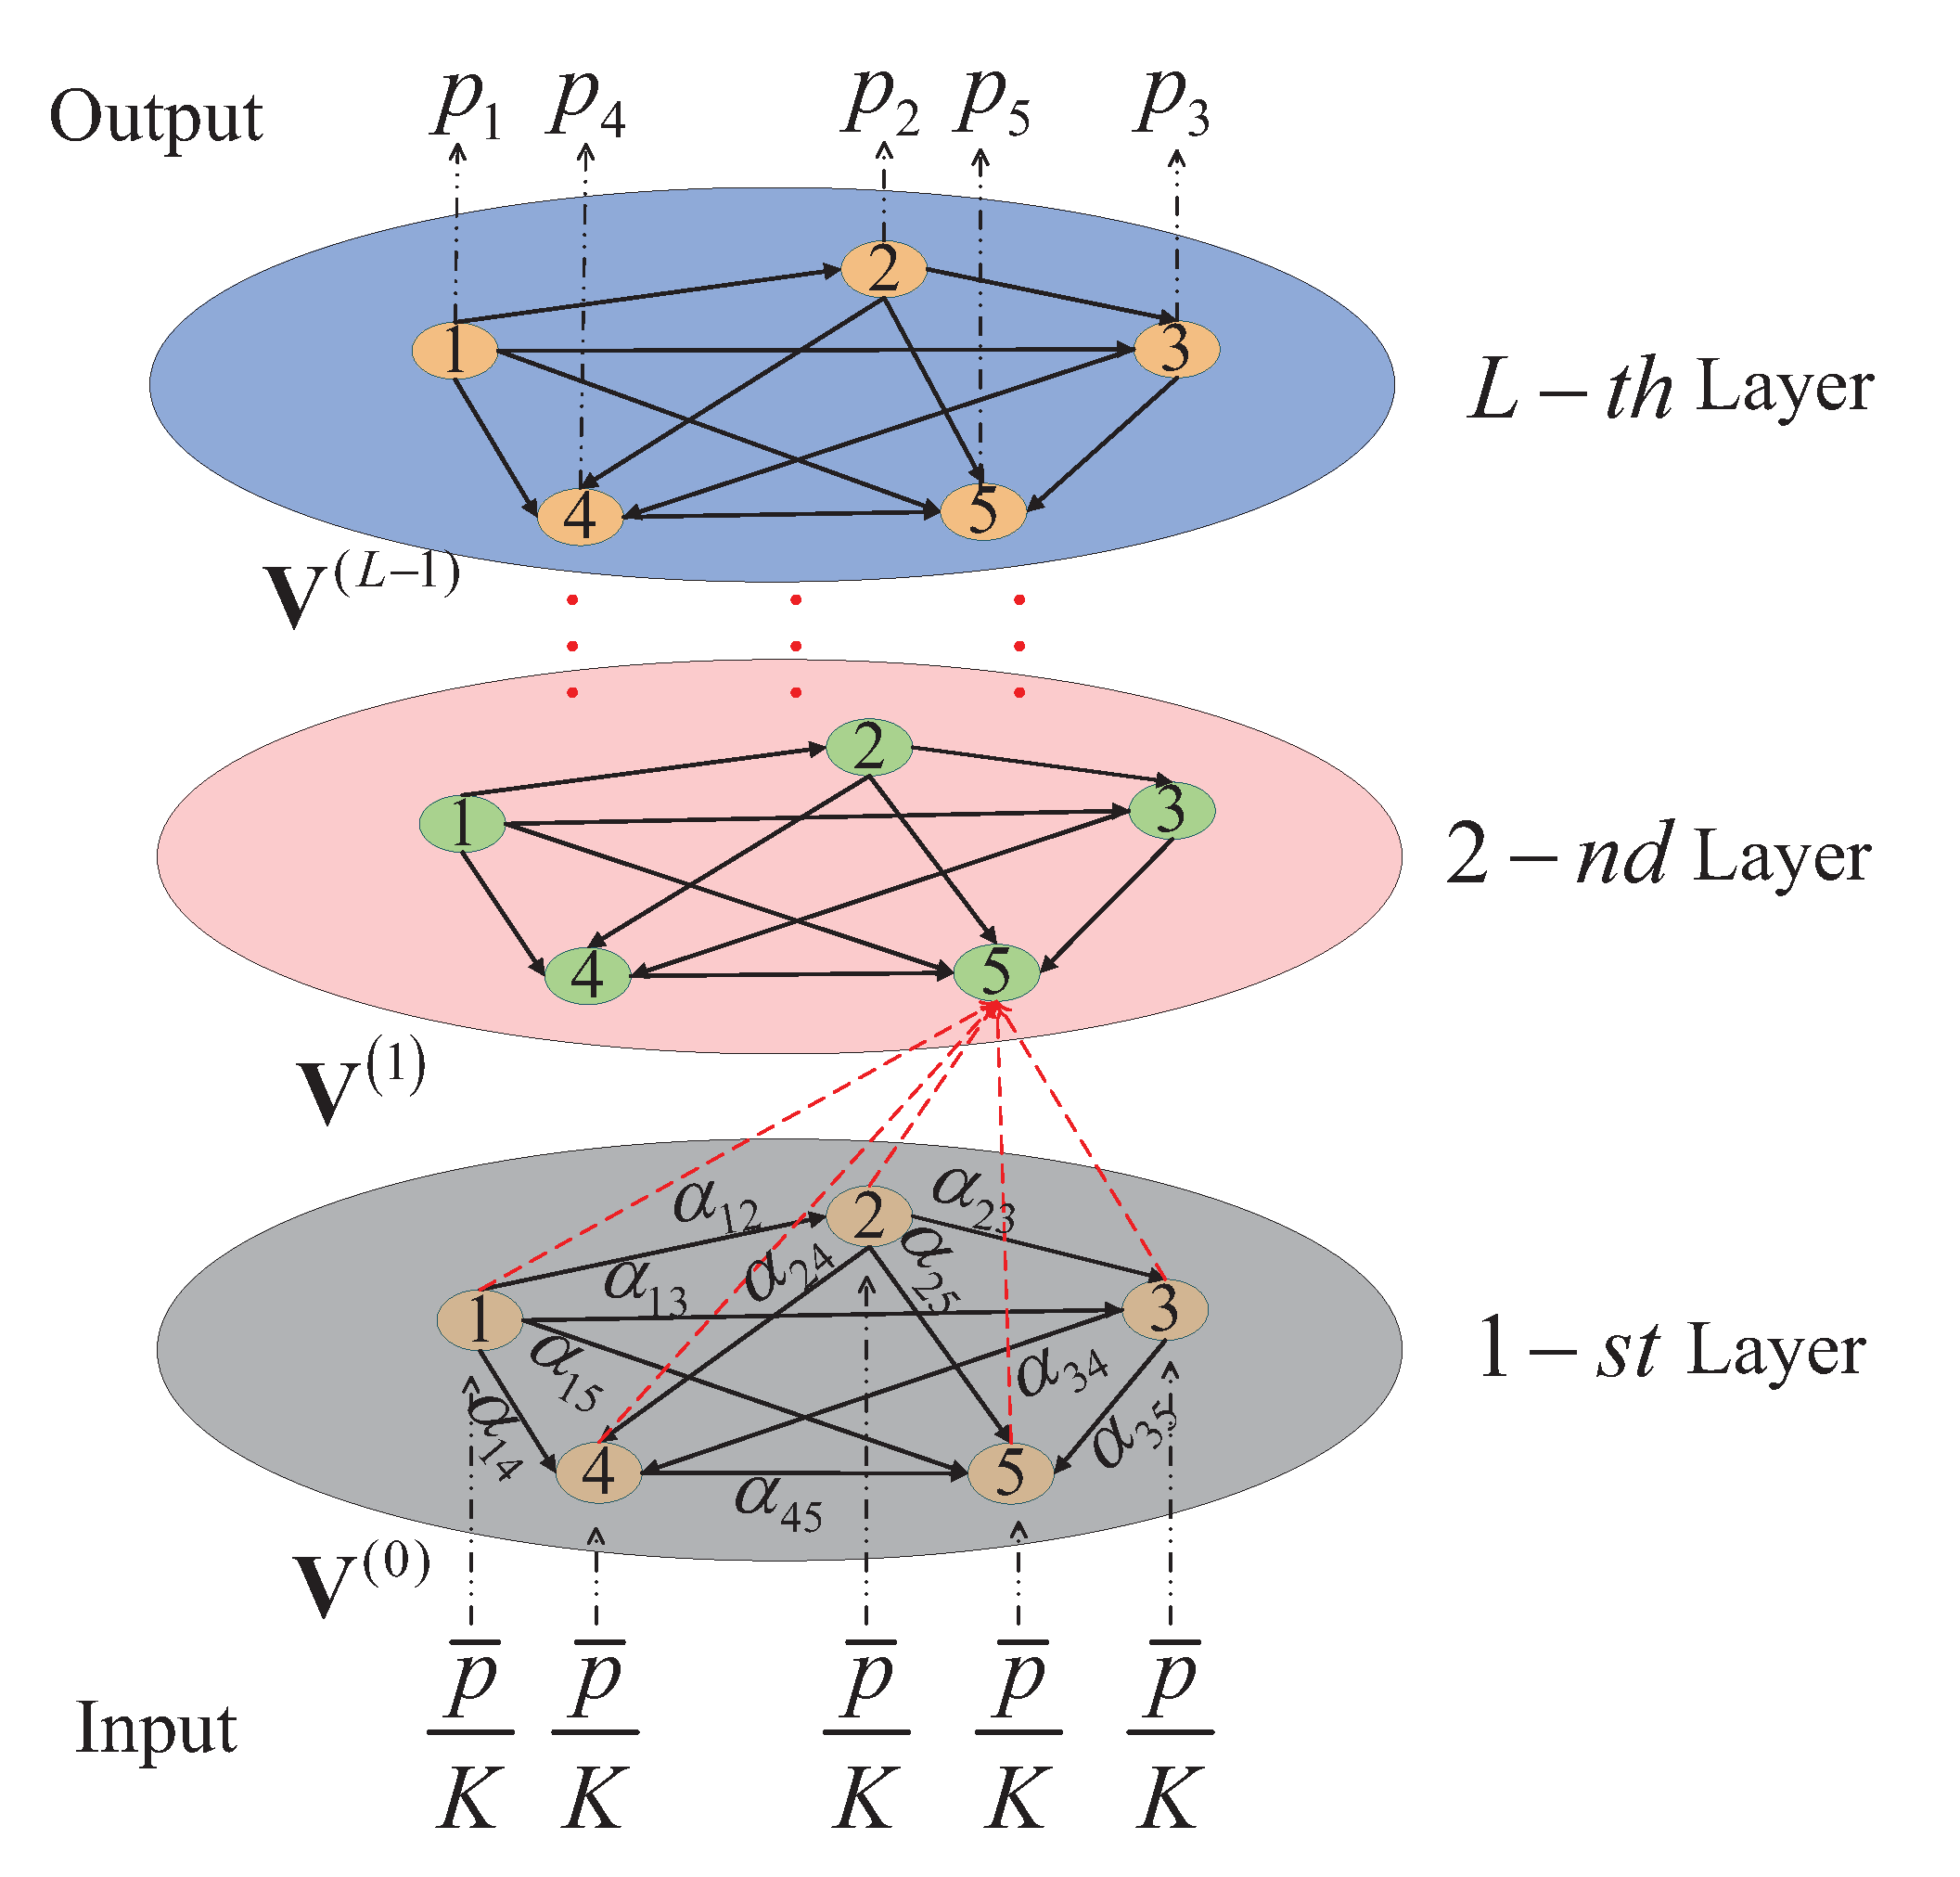
\includegraphics[width=8cm]{graphreprsent3.eps}
    \caption{A general $L$-layer GCN structure for the power-constrained HARQ schemes with $K=5$.} % 加参数进去
    \label{FIG2} %ÓÃÓÚÎÄÄÚÒýÓõıêÇ©
\end{figure}


%\begin{figure}[!htp]
%
%    \begin{minipage}[t]{1\linewidth}%É趨ͼƬÏÂ×ֵĿí¶È£¬ÔÚ´Ë»ù´¡¾¡Á¿Âú×ãͼƬµÄ³¤¿í
%    \centering
%    \includegraphics[height=2.4cm,width=3.8cm]{HARQ_system_model.eps}
%    \caption*{HARQ system schme}%¼Ó*¿ÉÒÔÈ¥µôĬÈÏǰ׺£¬×÷ΪͼƬµ¥¶ÀµÄ˵Ã÷
%    \label{FIG1}
%    \end{minipage}
%
%    \begin{minipage}[t]{0.5\linewidth}%ÐèÒª¼¸ÕÅÌí¼Ó¼´¿É£¬×¢ÒâÉ趨ºÏÊʵÄlinewidth
%    \centering
%    \includegraphics[height=2.4cm,width=3.8cm]{Grpahrepresent.eps}
%    \caption*{Transmission graph Representation}
%    \label{FIG2}
%    \end{minipage}
%    \caption{This is total name.}%nÕÅͼƬ¹²ÏíµÄ˵Ã÷
%\end{figure}

%Next, we briefly introduce the basic theory of GNNs, which learn good representations of vertices based on the topology of the data, node features, and edge connectivity features. Similar to CNN \cite{9155259,8335785}and MLP \cite{8444648}, GNN is also divided into a multi-layer structure. Each vertex aggregates the features of its domain vertices, and then the central node combines the features obtained by aggregation with its own features to update the representation of its own features. The update rule of node $v$ in the $l$-th layer is as follows
%\begin{equation}\label{eqn:gcnfunction}
%\begin{array}{l}
%\alpha _v^{(l)} = {\rm AGGREGATE}^{(l)}(\{ \beta _u^{(l - 1)}:u \in N(v)\} )\\
%\beta _v^{(l)} = {\rm COMBINE}^{(l)}(\beta _v^{(l - 1)},\alpha _v^{(l)})
%\end{array}
%\end{equation}
%where $\alpha _v^{(l)}$ is defined as the intermediate feature aggregated by node $v$ from its $l$th layer neighbors, and $N(v)$ is defined as the set of neighbor nodes of node $v$. $\beta _v^{(l)}$ represents the new representation of node $v$ after its $l$th level update.

%Therefore, different types of GNNs can be obtained by combining different $\rm AGGREGATE$ and $\rm COMBINE$ functions. Commonly used $\rm  AGGREGATE$ functions mainly include functions such as mean,max,min,sum. These functions are used to hope that this type of aggregation function has the characteristics of permutation invariance \footnote{is said to permutation invariance provided that $p_i^* = {f_i}(H,W) = {f_i}({\Pi ^T}H\Pi ,{\Pi ^T}W)$....
%For a given $i$, let ${f_i}\left( { \cdot , \cdot } \right)$ denotes the function that map the adjacency matrix and the weights to the optimal power allocation of the $i$-th transmission, i.e., $p_i^* = {f_i}(H,W)$ , and let $\Pi $ denote any permutation matrix}, that is, the input order of nodes will not affect the feature results of aggregation. For example, Graph Convolutional Network(GCN) commonly uses mean and relu as aggravation and combination functions, while Structure2Vec uses sum and relu.



\renewcommand{\algorithmicrequire}{\textbf{Input:}}  % Use Input in the format of Algorithm
\renewcommand{\algorithmicensure}{\textbf{Output:}} % Use Output in the format of Algorithm
\iffalse
\begin{algorithm}[h]
  \caption{GCN-Based Power Allocation Algorithm} % 名称
  \label{alg:algor1}
  \begin{algorithmic}[1]
    \Require
        The channel correlation coefficient $\rho$;
        The maximum number of transmissions $K$;
        The initial input power ${\bf V}^{(0)}$
    \Ensure
        The power allocation policy ${\bf V}^{(L)}$;
    \For {epoch $s=1,2,\cdots$}
        \State Sample a mini-batch from the dataset
        \State Apply GNN to learn the relationship
                between transmission nodes and then output power results
        \State Compute the variables' gradient of the  Lagrangian
        \State Update the primal variable $W_{s}$ according to \eqref{eqn:optweight};
        \State Update the dual variable $\lambda _{s}$ and $\upsilon _{s}$ according to \eqref{eqn:optstepa} and \eqref{eqn:optstepb};
    \EndFor
  \end{algorithmic}
\end{algorithm}
\fi

\begin{algorithm}[h]
    %\textsl{}\setstretch{1.8}
  \caption{GCN-Based Power Allocation Algorithm} % 名称
  \label{alg:algor1}
  \begin{algorithmic}[1]
    \Require
        Initial values $\bf W$, $\lambda$, $\upsilon$, ${\bf V}^{(0)}$
    \Ensure
        The power allocation policy ${\bf V}^{(L)}$;
    \For {epoch $s=1,2,\cdots$}
        %\State Sample a mini-batch from the dataset.
        \State Obtain  power allocation policy from a mini-batch.
        \State Compute the policy gradient of ${\cal L}({{\bf{W}}_s},{\lambda _s},{\upsilon _s})$.

        \State Update the primal variable $W_{s}$ [cf. \eqref{eqn:optweight}]:
        \Statex \hspace{0.68cm}${{\bf{W}}_{s + 1}} = {{\bf{W}}_s} - {\theta _{{\bf{W}},s}} {\nabla _{\bf{W}}}{{\rm E}_{\rho  \sim \mathcal A}}\left\{\mathcal L({{\bf{W}}_s},{\lambda_s} ,{\upsilon_s})\right\}$.

        \State Update the dual variable $\lambda _{s}$ and $\upsilon _{s}$ [cf. \eqref{eqn:optstepa}-\eqref{eqn:optstepb}]:

        \Statex \hspace{0.68cm}${\lambda _{s + 1}} = {\left[ {{\lambda _s} + {\theta _{{\lambda },s}}({{\rm E}_{\rho  \sim \mathcal A}}\left\{\log ({P_{out,K}})\right\} - \log (\varepsilon))} \right]_ + }$,
        \Statex \hspace{0.68cm}${\upsilon _{s + 1}} = {\left[ {{\upsilon _s} + {\theta _{{\upsilon },s}}({{\rm E}_{\rho  \sim \mathcal A}}\left\{p_{\rm avg}\right\} - \bar p)} \right]_ + }$.
    \EndFor
  \end{algorithmic}
\end{algorithm}


\section{Numerical Experiments}\label{sec:EXPERIMENTS}
Numerical experiments are conducted for verification in this section. %The simulation of three types of HARQ using GCN as the parameter optimization method.
For illustration, we assume that ${\xi _1} =  \cdots =  {\xi _K} = 1$, $\delta  = 1$, $K=3$, $R = 2$ bps/Hz, $N_b=10^6$~bits, $B=10$~MHz, and $\varepsilon = 10^{-2}$. With regard to the neural network structure, a $5$-layer GCN with intermediate feature dimensions 16, 32, 16 and 2 is implemented. The activation functions $\sigma ( \cdot )$ in the intermediate layers use ``\emph{ReLU}'', while the last layer applies ``\emph{Linear}''. A dataset with 1000 samples is used in the training stage, the total number of training epochs is set to $500$, and the learning rates of ${\theta _{{\bf{W}},s}}$, ${\theta _{\lambda,s}}$, and ${\theta _{\upsilon,s}}$ are assumed to be $5 \times {10^{ - 4}}$, $10^{-3}$ and $5 \times {10^{ - 5}}$, respectively. The GCN parameters $\bf W$ are updated by using the adaptive moment estimation (Adam) optimizer. Besides, the expectations in \eqref{eqn:optweight} - \eqref{eqn:optstepb} are taken over the sampled mini-batch of size 50, and $\rho $ is randomly generated from a uniform distribution within the interval $\left[ {0,1} \right)$. %By considering the unit average noise power, the average total transmit SNR is defined as ${\textsc{snr}} = \bar P$.

In Fig. \ref{FIG7}, the convergence of the primal-dual learning algorithm for three HARQ schemes is investigated by setting $\bar p = 15$~dBW. Clearly from Fig. \ref{FIG7}, the proposed algorithm can converge within $1200$ iterations, which justifies the effectiveness of the GCN-based power allocation strategy. If the maximum power constraint $\bar p$ is sufficiently large (e.g., 15~dBW), the LTAT converges to the predefined transmission rate $R=2$~bps/Hz. Hence, it is observed from Fig. \ref{FIG7} that the latency approaches to $N_b/(B\eta)=10^6/(10^7\times 2)=0.05$~s with the increase of the number of iterations.

% {\color{red}{pay attention to the unit of $\bar p\to $dBW}, use $\bar p$  instead of SNR}

\begin{figure}[htbp]
    \centering
    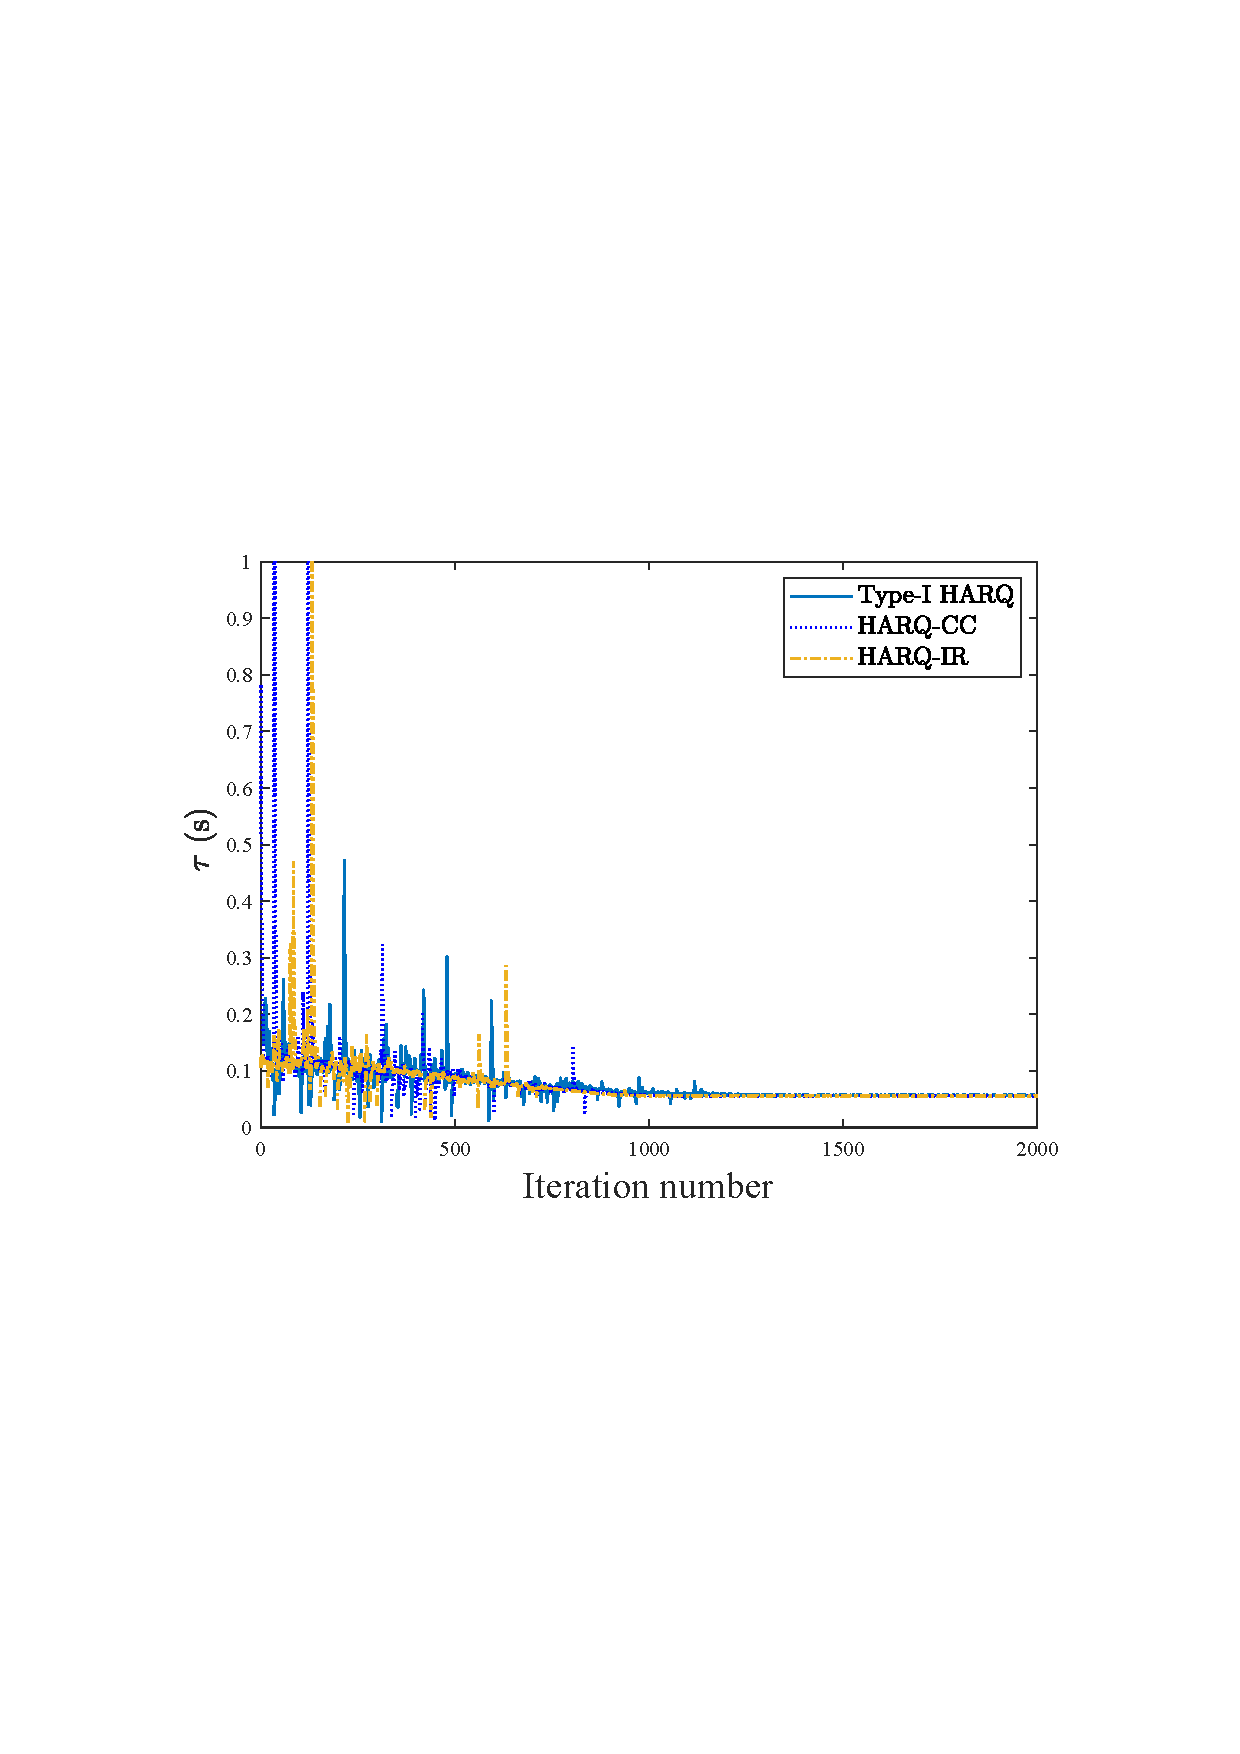
\includegraphics[width=8cm]{delay-itera7.pdf}
    \caption{The convergence analysis of the primal-dual learning algorithm with respect to the number of iterations.}
    \label{FIG7} %ÓÃÓÚÎÄÄÚÒýÓõıêÇ©
\end{figure}

%For the channel model part, we follow the settings in the paper \cite{8171001}, namely .
%For the neural network layer part, we set the power distribution network as a $5$-layer GCN with intermediate feature dimensions , the activation function $G ( \cdot )$ of the intermediate layer adopts ``$\rm relu$'' and for the last layer we apply a ``$\rm linear$'' layer. The number of training epochs is $500$ and the learning rate is set to $10^{-3}$.

%First, we tested the feasibility of using GCN as a parameter optimizer. In Fig. \ref{FIG7}, The throughput showed a gradual increase as the number of iteration rounds increased, and the number of iterations stabilized at about $300$ rounds due to the accurate capture and learning ability of the graph neural network for structural information.



%We tested the effect of the GCN power optimizer under different maximum power ${\bar P}$ dB if $\rho=0.5 $. The results are shown in Fig. \ref{FIG3} and \ref{FIG4},  which show the changes of HARQ system throughput and outage probability, respectively. From the above two figures, In the case of low SNR, HARQ-IR shows better performance among the three schemes. Compared with TYPE-I, HARQ-CC performs better due to the introduction of diversity gain. Compared with HARQ-CC, HARQ-IR adds additional Coding gain shows better performance. At the same time, LTAT can be improved by increasing SNR, but LTAT of all HARQ-aided schemes tends to be fixed at high SNR, According to (\ref{eqn:throught2}), as the value of the given SNR increases, the power allocated to each round of transmission increases and the probability of outage decreases, thus it is easy to conclude that the magnitude of the throughput value is close to the transmission rate in the case of high SNR.

In Figs. \ref{FIG4} and \ref{FIG3}, the minimal latency and the corresponding outage probability are plotted against the total average transmit power $\bar p$, respectively, where $\rho=0.5 $ is considered. It is not beyond our expectation from both figures that HARQ-IR performs the best, followed by HARQ-CC, and the worst is Type-I HARQ. Moreover, it can be seen from Fig. \ref{FIG4} that a significant latency reduction can be achieved by HARQ-IR under a small $\bar p$ when compared to the other two HARQ schemes. In addition, it can be observed from Figs. \ref{FIG4} and \ref{FIG3} that there is no feasible solution for Type-I HARQ and HARQ-CC under a sufficiently low transmit power. However, under a large power constraint, e.g., $\bar p>16$~dBW, the latency curves of three HARQ schemes almost coincide with each other. Hence, the superior performance of HARQ-IR in terms of the low latency is weakened as $\bar p$ increases. %a negligible performance gap between the HARQ schemes can be observed,
Nevertheless, it can be seen from Fig. \ref{FIG3} that HARQ-IR still has a notable outage reduction compared to the other two schemes. Moreover, as $\bar p$ increases, the latency is lower bounded by 0.05~s, which has been illustrated in Fig. \ref{FIG7}. Whereas, the corresponding outage probabilities of three HARQ schemes continuously decline with $\bar p$.

\begin{figure}[htbp]
    \centering
    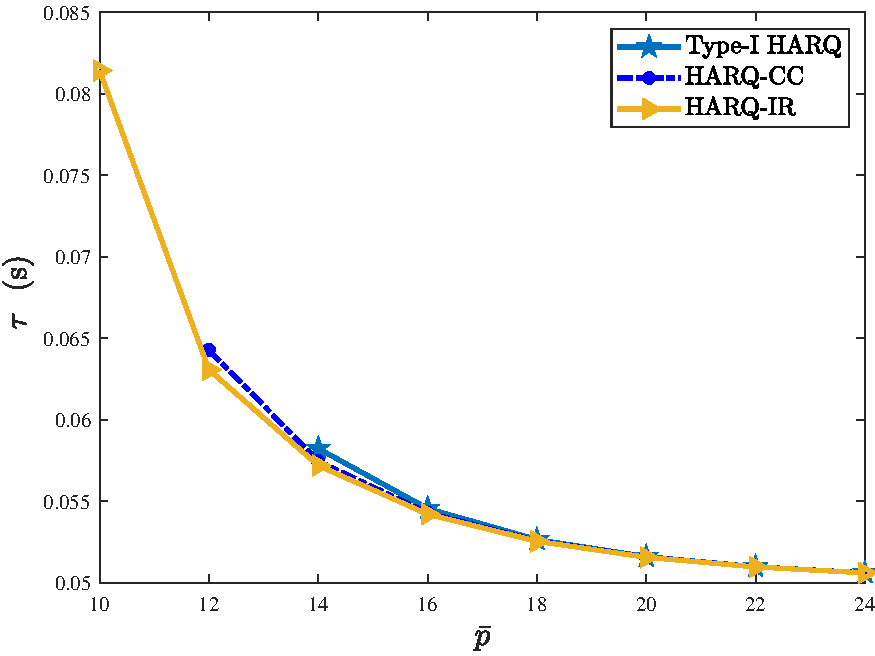
\includegraphics[width=8cm]{power-delay.pdf}
    \caption{The comparison between the latency of different HARQ
schemes.}
    \label{FIG4} %ÓÃÓÚÎÄÄÚÒýÓõıêÇ©
\end{figure}

\begin{figure}[htbp]
    \centering
    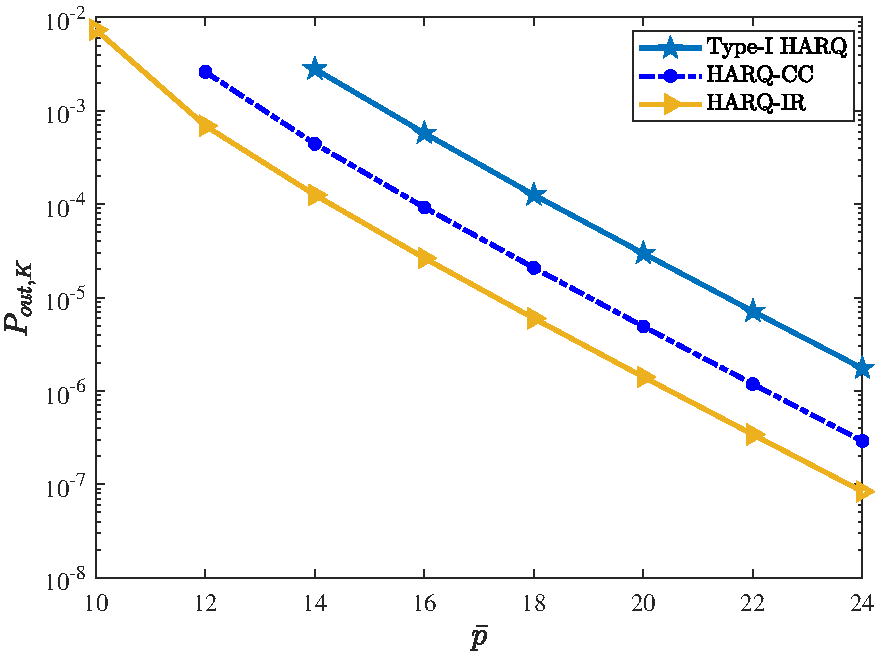
\includegraphics[width=8cm]{power-outage.pdf}
    \caption{The comparison between the outage probabilities of different
HARQ schemes.}
    \label{FIG3} %ÓÃÓÚÎÄÄÚÒýÓõıêÇ©
\end{figure}
As shown in Figs. \ref{FIG5} and \ref{FIG6}, the effects of the time correlation on the latency and the outage probability are respectively examined by fixing ${\bar p}=15$~dBW. It is consistent with the observations in\cite{7448651,7833558,7959548} that the time correlation has a negative impact on the latency and outage performance. For example, as the time correlation increases from 0 to 0.98, the latency of HARQ-IR increases from 0.0554s to 0.0564s, and the corresponding outage probability of HARQ-IR decreases from $5.76 \times {10^{ - 5}}$
 to $1.68 \times {10^{ - 3}}$. Moreover, when the HARQ channels undergo a slightly correlated fading, i.e., $\rho<0.5$, the impact of the time correlation on the latency and the reliability can be disregarded. To sum up, HARQ-IR has the superior performance to offer low latency while ensuring high reliability, albeit at the price of extra coding complexity.%${\cal L}(\rho ,K)$ of (\ref{eqn:pout_asy}) is a decreasing function of time correlation coefficient $\rho$. As the correlation coefficient increases, the outage probability gradually increases and the throughput performance decreases. The results in the figure show that time correlation has a negative impact on outage probability and throughput.

\begin{figure}[htbp]
    \centering
    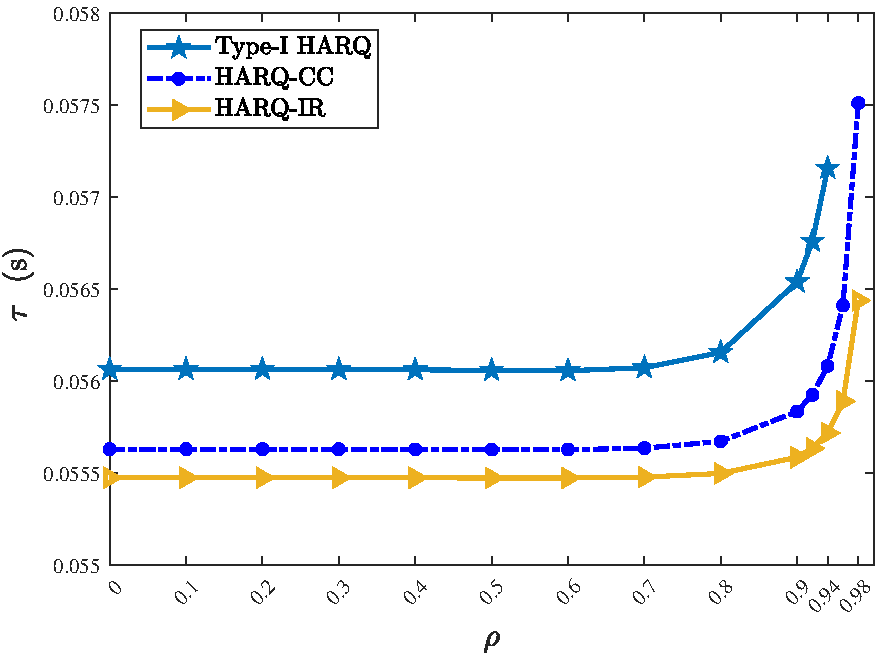
\includegraphics[width=8cm]{factor-delay1.pdf}
    \caption{Effect of the time correlation on the latency.}
    \label{FIG5} %ÓÃÓÚÎÄÄÚÒýÓõıêÇ©
\end{figure}

\begin{figure}[htbp]
    \centering
    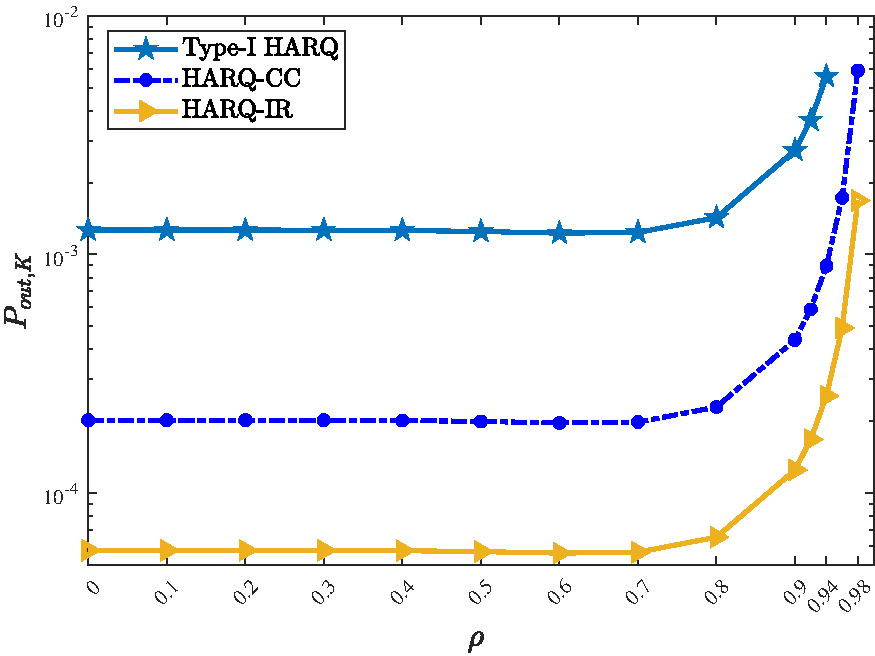
\includegraphics[width=8cm]{factor-outage1.pdf}
    \caption{Effect of the time correlation on the outage probability.}
    \label{FIG6} %ÓÃÓÚÎÄÄÚÒýÓõıêÇ©
\end{figure}




\section{Conclusion}\label{sec:CONC}
This paper studied the power-constrained HARQ schemes for realizing URLLC. More specifically, the transmission latency of HARQ schemes was minimized while guaranteeing the high reliability and limited power consumption. To render the optimization tractable, the asymptotic outage expression was used. By considering the intricate relationship between different HARQ rounds, the GCN was invoked to enable the latency minimization problem owing to its capability of tackling the graph data. The primal-dual learning method was then leveraged to train GCN parameters. Finally, the numerical experiments were performed to corroborate the validity of the proposed power-constrained HARQ schemes and compare the latency and reliability performance among three HARQ schemes. %HARQ-IR has the superior performance to offer low latency while ensuring high reliability, albeit at the price of high coding

%We study the problem of using HARQ-IR to allocate transmission power to maximize throughput in time-correlated fading channels, changing its optimization process from traditional methods to using graph neural networks to capture node relationships in the transmission process to optimize the problem. From the above results, it is proved that the proposed method based on graph topology learning can select results with lower outage probability and better throughput results under different power constraints.

\bibliographystyle{IEEEtran}
\bibliography{reference}
\end{document}


